\chapter{Hardware}
The setup of the manipulator was a 3D camera mounted above the manipulator to view its workspace. A micro-controller and computer were the main methods of control. The manipulator control system is set up as seen in the diagram in Figure \ref{fig:maindiagram}. Camera data is read in and processed by the computer, the results are sent to the micro controller, which sends PWM signals to the servo motors through a power and control circuit. A diagram of connections within this system can be seen in Figure \ref{fig:diagram} The code to handle the communication of the system can be found in Appendix B.

\begin{figure}[h]
\centering
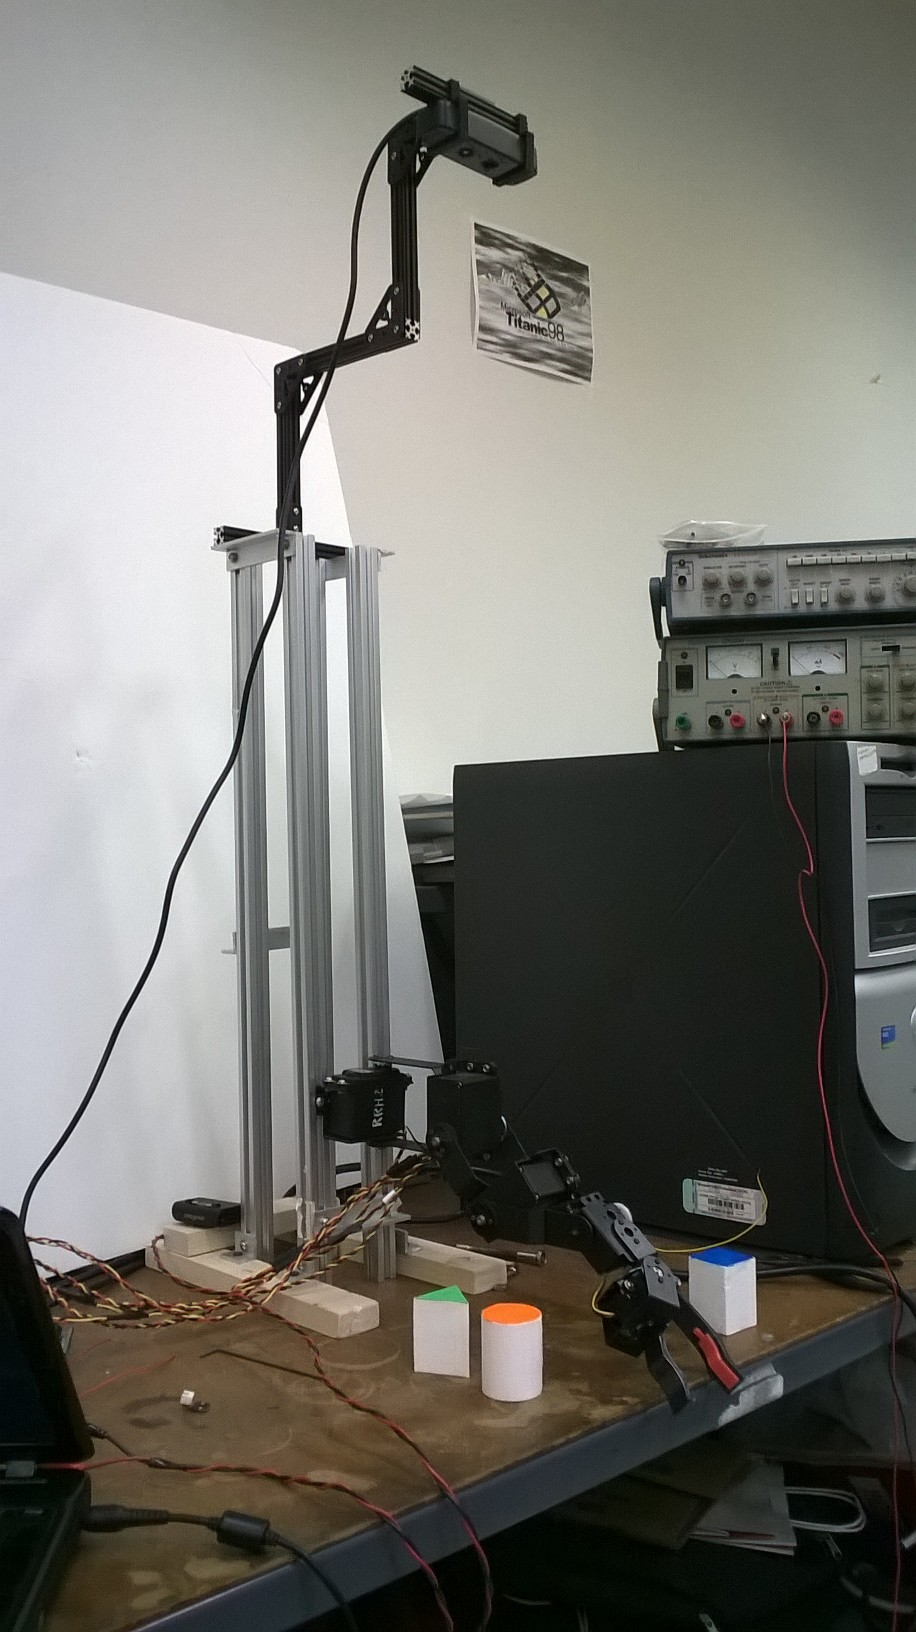
\includegraphics[height=0.5\textwidth]{actual}
\caption{The manipulator.}
\label{fig:real}
\end{figure}

\begin{figure}[h*]
\centering
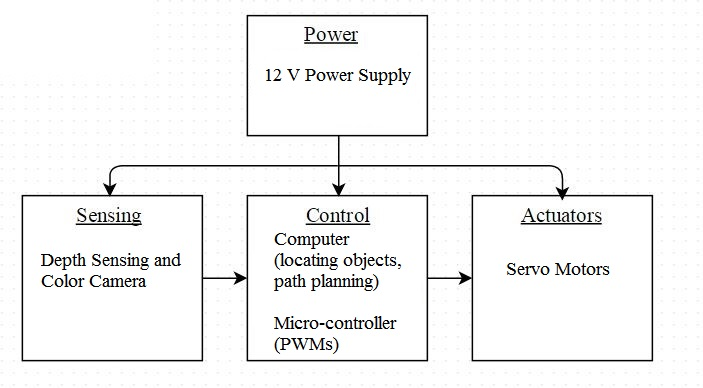
\includegraphics[width=0.7\textwidth]{maindiag}
\caption{System diagram of the manipulator.}
\label{fig:maindiagram}
\end{figure}

The servos used to construct this arm had no method of feedback. The connections of each servo were power, ground, and input signal. Unlike some more expensive servos which have a connection for some or multiple types of feedback these servos are operated as a feed forward system. This means that commands that are given are not adjusted by any kind of error provided by a feedback system. The code on the micro controller for controlling these servos can be seen in Appendix C.


\begin{figure}
\centering
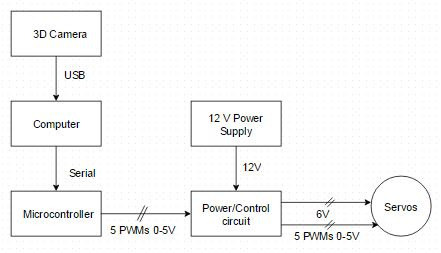
\includegraphics[width=0.6\textwidth]{diagram}
\caption{Diagram of manipulator control system.}
\label{fig:diagram}
\end{figure}

The camera used was a Creative Senz 3D depth sensing and color camera. The computer code was run on Linux using bot C++ and Python. The micro controller used was a small lab built autopilot. The processor on the autopilot was a TM4C controller. The TM4C was used to control the servos. This code was originally designed on an RM48 processor but switched over to make future integration with a mobile platform robot easier. The manipulator itself is constructed from Hitec servos and the associated brackets. A list of all components can be found in Table \ref{tab: Components}.

\begin{longtable}{| p{3cm} | p{10cm} |}
		\caption{List of major components on the robotic manipulator system.}
		\label{tab: Components}\\

 		\hline
 		 Component & Description \\ \hline 
 		\endhead
 		

 		
 		\hline \hline
 		\endlastfoot
 		
 		Baby Autopilot(BAP) & Small single processor control unit. 
	 		\\ & $ \bullet $ 80 Mhz TM4C123GH6PZ micro-controller with 32 kB internal RAM and 256 kB internal Flash  
	 		\\  & $ \bullet $ 2 UARTs  
 			\\  & $ \bullet $ 8 PWM outputs	
 		\\ \hline
		Camera & USB Color and Depth Sensing camera
			\\  & $ \bullet $ USB 2.0 and USB 3.0 compliance
	 		\\  & $ \bullet $ Max frame rate of 30fps
	 		\\  & $ \bullet $ Depth range from 6 in to 3 ft. 
 		\\ \hline

 		Servos & Servo motors  
 			\\  & $ \bullet $ Pulse Width Control 1500usec Neutral
 			\\  & $ \bullet $ 6V operating voltage
 			 			 			 		
 		\\ \hline 
	\end{longtable}
%\end{table}

The power/control circuit is mostly a 6-volt regulator with connections between the servos and micro controller. The layout is shown in Figure \ref{fig:circuit}. An enable pin and jumper were used so that the servos only receive power when an enable signal, GPIO of 3.3v, is sent from the micro controller. The jumper can also be removed to stop powering the servos in the case power needed to be shut off quickly.

\begin{figure}[h]
    \centering
    \begin{subfigure}[b]{0.3\textwidth}
    	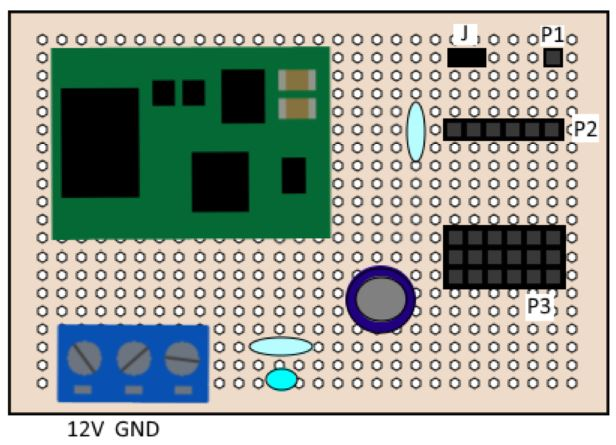
\includegraphics[width=\textwidth]{circuit}
   	 \end{subfigure}
   	 \quad

 %add desired spacing between images, e. g. ~, \quad, \qquad, \hfill etc.
      %(or a blank line to force the subfigure onto a new line)
 	\caption{Connection Circuit for Manipulator. }
 	\label{fig:circuit}
\end{figure}

The last major design component for the hardware was the manipulator's gripper. It was built from a combination of a Hitec servo, existing brackets, and 3D printed pieces. The design concept was a fixed thumb with an opening and closing finder controlled by the servo. All parts were modeled in Solidworks and the thumb and finger pieces printed. Rubber was glued onto the 3D printed pieces to increase the friction when picking up objects. The assembly of the gripper opened and closed around a cylindrical object is shown in Figure \ref{fig:gripper}. The object and similar objects were also 3D printed and used as the goal and obstacles for the arm.

\begin{figure}[h]
\centering
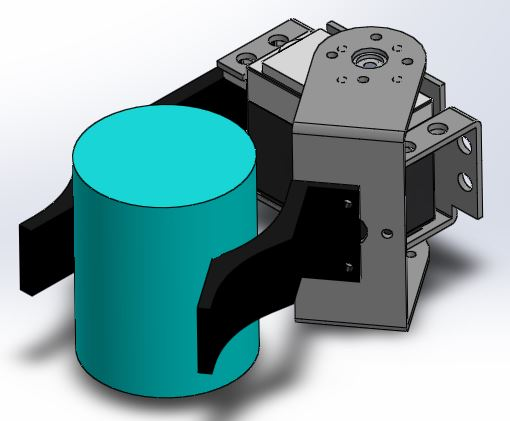
\includegraphics[width=0.4\textwidth]{gripper}
\caption{Gripper holding cylindrical object.}
\label{fig:gripper}
\end{figure}